\part{Introdução e Referêncial Teórico}

\chapter[Introdução]{Introdução}
% \addcontentsline{toc}{chapter}{Introdução}




% tema e contexto
\section{Contexto e introdução teórica}
No cenário de desenvolvimento de software atual, é praticamente obrigatório o uso de ferramentas de versionamento, seja para código, configurações ou para documentação em geral \cite{version_control_git}.

O uso de sistemas e técnicas de versionamento e revisão de versões se tornaram essenciais para o desenvolvimento de software atualmente.
Tais sistemas são encontrados em três diferentes paradigmas: sistemas de versionamento local, sistemas de controle de versão distribuídos - \textit{DVCS} - e sistemas de controle de versão centralizados - \textit{CVCS} \cite{version_control_review}.

Com a contínua expansão da comunidade de software livre, se tornou cada vez mais comum o uso de sistemas DVCS por conta das desvantagens ou impedimentos que os outros paradigmas proporcionavam para o desenvolvimento colaborativo \cite{version_control_review} \cite{version_control_git}.


Inserido neste cenário, o \textit{Git} é uma das ferramentas mais poderosas e utilizadas pelos desenvolvedores de software espalhados mundo afora \cite{git_version_cookbook}. O \textit{Git}, é um software de versionamento de arquivos no formato distribuído criado por Linus Torvalds
% para o desenvolvimento do \textit{kernel Linux} 
e se tornou recentemente a principal tecnologia utilizada para versionamento de repositórios de software \cite{openhub_git_svn}, como demonstra o gráfico de comparação de repositórios tirado do OpenHub (Figura \ref{Fig_comparisson_git}).
De um espaço amostral de 1.296.669 repositórios, aproximadamente 70\% são versionados utilizando o Git, sendo que o Subversion - ou SVN - a segunda maior tecnologia, é utilizado em aproximadamente 25\% dos mesmos.


\begin{figure}[h]
    \centering
    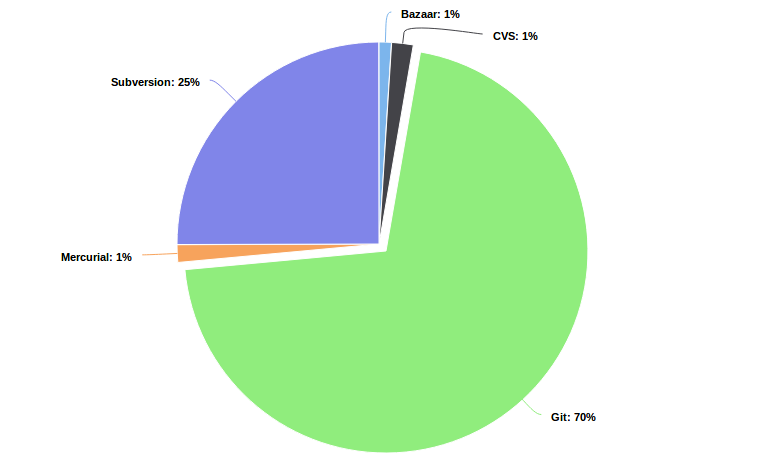
\includegraphics[width=16cm]{figuras/git_svn_comp.png}
    \caption{Comparação de número de repositórios com o Git e outras tecnologias. Fonte: \textit{openhub}}
    \label{Fig_comparisson_git}
\end{figure}

O Git é um software livre que segue a filosofia \textit{FLOSS} e, provavelmente por conta disto, possui uma vasta gama de ferramentas em seu ecossistema a fim de dar suporte ao desenvolvedor.
Além de várias CLIs e UIs voltadas para a ajuda no uso da ferramenta, existem os gerênciadores de repositórios do Git \cite{building_tools_github}. 

Estes gerenciadores são plataformas no qual são submetidas as alterações dos repositórios, sendo as mais utilizadas o \textit{Github}, \textit{GitLab} e \textit{Bitbucket}. Com o uso destas ferramentas, o já presente suporte ao desenvolvimento colaborativo no git se torna mais significante, visto que elas proveêm suporte para diversas formas de organização e distribuição de tarefas para equipes, além de diversas integrações com ferramentas externas. 

% Tal suporte à colaboração não é algo novo, visto que existe desde a concepção do Git por Torvalds \cite{version_control_git}, visto que era um requisito novo e necessário a capacidade de suportar trabalho distribuído e tratar de alterações no mesmo trecho de código. Na realidade atual, tal capacidade é cada vez mais necessária com times de desenvolvimento se tornando cada vez mais distribuídos \cite{developer_survey}.



Tal suporte fez com que as comunidades de software livre utilizassem dessas plataformas para manter seus projetos \textit{open-source} abertos para contribuições externas, de uma forma mais acessível e - em geral - menos burocrática. Considerando o fato de times de desenvolvimento cada vez mais distribuídos estarem se tornando uma realidade progressivamente mais comum \cite{developer_survey}, é possível afirmar que a demanda para plataformas colaborativas é sólida e não deixará de ser significante facilmente.

Com a popularização destas plataformas e do workflow envolvido para a contribuição em softwares livres, começaram a surgir diferentes tipos de documentação, regras e guias voltados à auxiliar desenvolvedores a contribuírem em projetos, mantendo ao mesmo tempo a organização e qualidade dos mesmos.

Seja essa documentação composta dos clássicos  guias de contribuição e \textit{READMEs}, até os novos templates de \textit{pull request}, \textit{issues}, é essêncial que essa documentação exista para guiar novos contribuidores.

Pensando nisso, o Github lançou o dashboard de ferramentas para comunidade em 14 de junho de 2017 \cite{post_github_community_tools} proporcionando recomendações de documentação consideradas como boas práticas para repositórios de software livre, esse dashboard pode ser visto na aba \textit{insights} opção \textit{community}, conforme a figura \ref{Fig_dash_community}.


\begin{figure}[h]
    \centering
    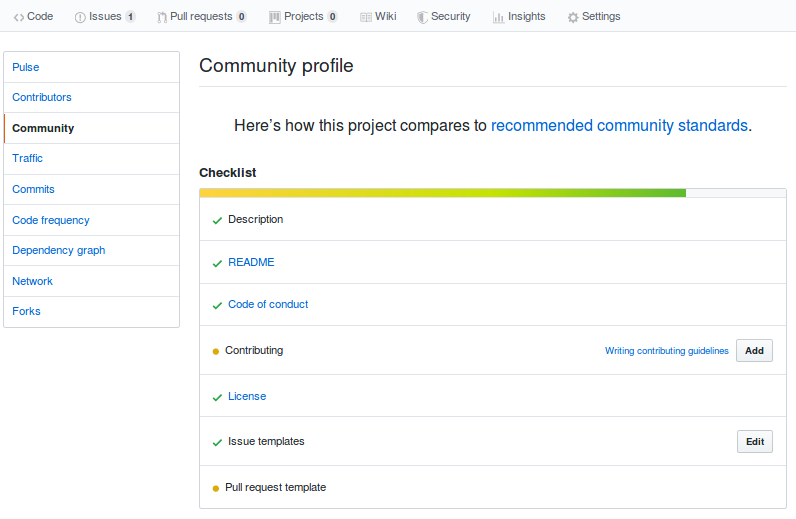
\includegraphics[width=16cm]{figuras/min_dashboard_community.png}
    \caption{Exemplo de dashboard de comunidade no Github}
    \label{Fig_dash_community}
\end{figure}

Segundo essas recomendações, um bom repositório de software livre deve possuir pelo menos os seguintes artefatos \cite{opensource_guidelines_github}:

\begin{itemize}
    \item Descrição do repositório
    \item Arquivo README
    \item Código de conduta
    \item Guia de contribuição
    \item Licença
    \item Template de \textit{issue}
    \item Template de \textit{pull request}
\end{itemize}

Embora aparentemente tenha tomado para si o papel de guia do desenvolvimento \textit{open-source}, por conta de ser a maior e mais usada plataforma de host de repositórios no mundo, não são todos que seguem estas recomendações do Github.
Outras plataformas atualmente não possuem este mesmo recurso de dashboard ou guias como os presentes no Github. Nelas estes são inexistentes ou não se encontram de forma explícita.

Um dos maiores pontos de divergência entre as comunidades de desenvolvimento é o que são consideradas boas práticas e boas políticas de repositório. Existem diversas 'fraturas' acerca do que comunidades de desenvolvimento definem sobre o que é ou não uma boa prática. Por exemplo, o guia de projetos open-source do github define uma checklist de elementos que um bom repositório de software livre deve possuir \cite{opensource_checklist_github}, já a Linux Foundation define uma outra checklist \cite{opensource_checklist_linux_foundation}, possuindo diferentes elementos entre um e outro.

Sejam essas diferenças relacionadas aos commits durante o desenvolvimento de um projeto ou à mínima documentação necessária para um repositório de software livre, a realidade é que existem diversas opiniões - algumas até conflitantes - sobre o assunto.

Ao mesmo tempo que essa ampla gama de opiniões é algo capaz de provocar confusão para o desenvolvedor, ela também provê diferentes experiências e possibilidades de abordagem. Tal flexibilidade é algo notório principalmente considerando a popularidade de metodologias ágeis no cenário de desenvolvimento de software atual, e inclusive a importância que estas mesmas dão para a experimentação e empiricidade em seus processos de desenvolvimento.








\section{O problema}
% o problema
Com tamanha diversidade de padrões, convenções e formatos, é comum que exista bastante inconsistência dentro dos repositórios e projetos de software. Este fato pode ocorrer por vários fatores, sendo o principal deles a adaptação à um contexto diferente de desenvolvimento.

Tal adaptação é custosa de tempo e a adaptabilidade necessária de um desenvolvedor à um contexto de trabalho é um requisito do mercado cada vez mais cobrado. Essa adaptação se torna mais custosa na mesma proporção da quantidade de regras e políticas adotadas na equipe de desenvolvimento.

Uma forma simples de se perceber isso é olhando a árvore de commits - \textit{commit tree} - de um projeto de software. Mesmo com diversas boas práticas de escrita de commit diferentes documentadas, muitos desenvolvedores desconhecem ou não aplicam. Ou no caso dessas boas práticas serem aplicadas e exigidas, caso venha a se ter um novo membro na equipe, a curva de aprendizado dele será impactada.

Uma solução para esses problemas necessitaria de, ao mesmo tempo, ser adaptável para lidar com diferentes padrões e contextos, e ser corretiva além de capaz de guiar a aplicação de boas práticas de acordo com os mesmos.









% objetivos
\section{Objetivos}
Este trabalho tem como objetivos:

\begin{itemize}
    \item Identificar os principais padrões e boas práticas utilizadas em um espaço amostral de repositórios do Github e Gitlab. 
    \item Analisar os padrões e levantar suas características.
    \item Implementar uma ou mais ferramentas capazes de resolver o problema levantado.
\end{itemize}

O espaço amostral citado no primeiro item consistirá dos 5 maiores repositórios de software livre no Github assim como 5 do Gitlab, 5 repositórios de software livre de pequeno a médio porte também presentes em ambas as plataformas e, por fim, 5 repositórios de software livre recentemente criados, totalizando uma amostra de 25 repositórios.

